%OBAL
\thispagestyle{empty}
\begin{center}
  \textsc{ 
    {\Large \school\\ \faculty}
    \vfill
    {\LARGE \title}\\ \vspace{0.5cm}
    {\large \thesis}
  }
\end{center}
\vfill

\begin{flushleft}
  \year\\
  \hspace{0.5cm} \author
\end{flushleft}


%TITULNY LIST
\thispagestyle{empty}
\begin{center}
  \textsc{ 
    {\Large \school\\ \faculty}
    \vfill
    {\LARGE \title}\\ \vspace{0.5cm}
    {\large \thesis}
  }
\end{center}
\vfill

\begin{flushleft}
  \begin{tabular}{@{}ll}
    Study programme: & \studyprogramme \\
    Study field: & \studyfield \\
	  Department: & \department \\
    Supervisor: & \supervisor
  \end{tabular}
  \vspace{1cm}

  \placeandyear\\
  \hspace{0.5cm} \author
\end{flushleft}



\shorthandoff{-} %docasne deaktivuje znak '-' v balicku babel
%ZADANIE EN
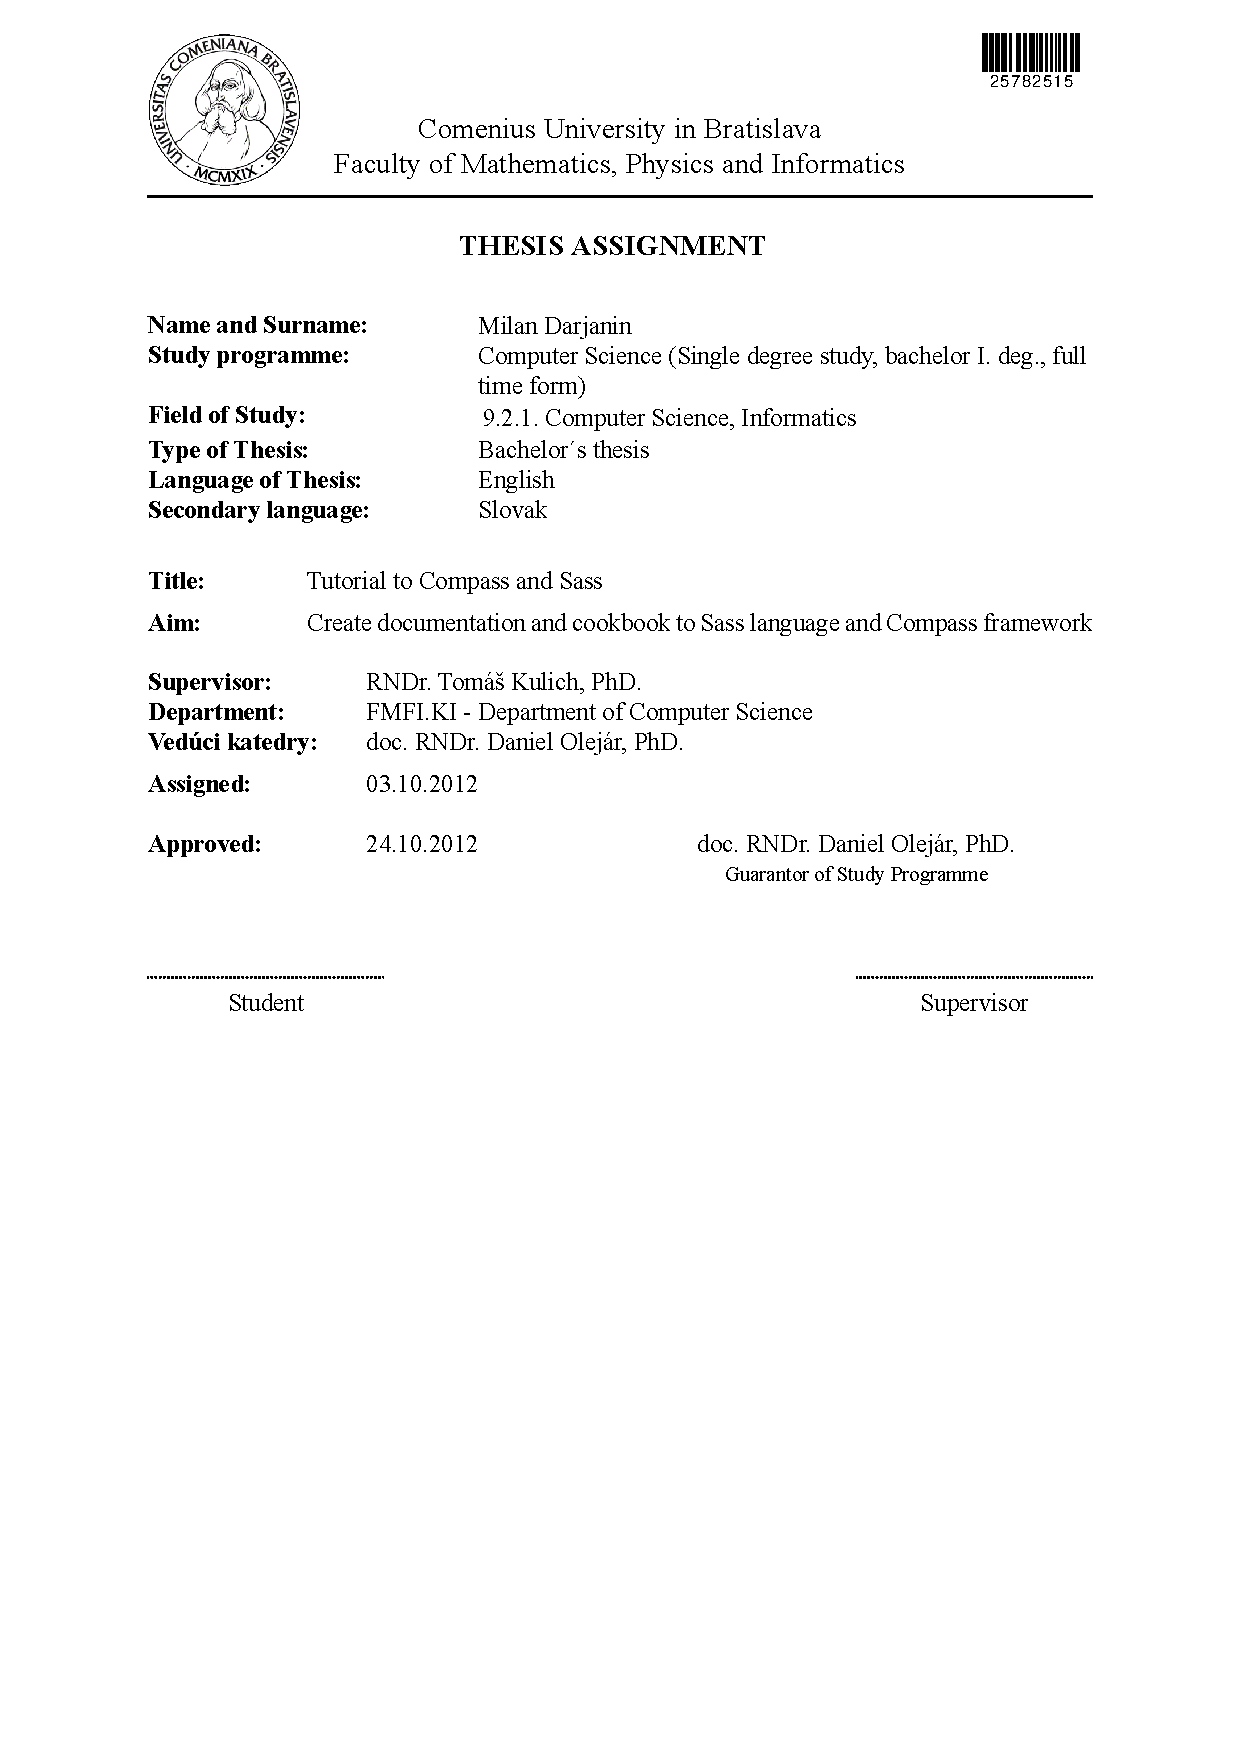
\includepdf[pages=-]{frontmatter/assignment.pdf}
%ZADANIE SK
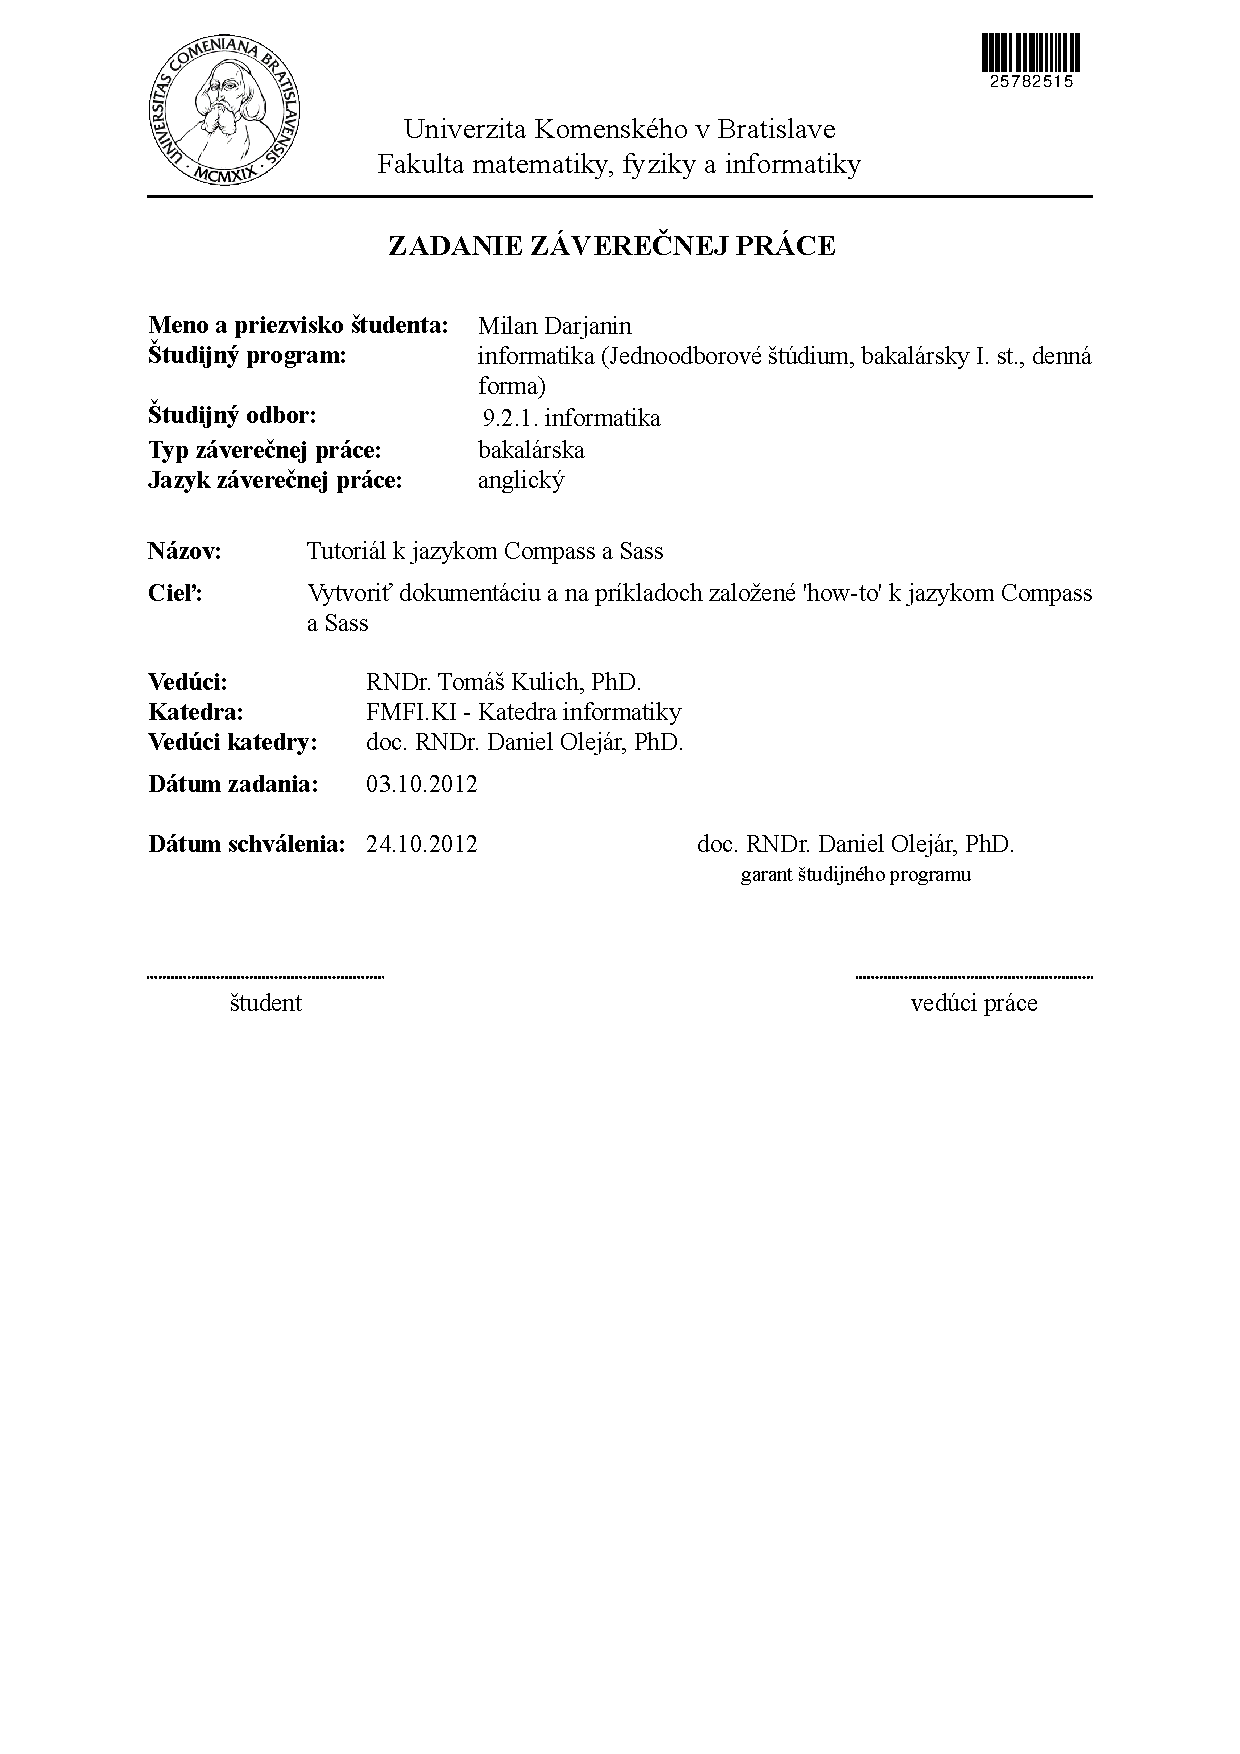
\includepdf[pages=-]{frontmatter/zadanie.pdf}
\shorthandon{-}

%PODAKOVANIE
\chapter*{Acknowledgement}
\vfil
I would like to thank my supervisor \supervisor for his help and advices.


%ABSTRAKT EN
\chapter*{Abstract}
The goal of the first chapters is to teach a reader a syntax and features of the preprocessor SASS. The following chapters are devoted to framework Compass, which is targeted to speed up development of projects. More about it is in chapters 3, 4 and 5. The last part is giving practical examples written in SASS using Compass, that can be used in real-life projects. The complete text has online version at darjanin.com/sass-tutorial. The source codes for examples are located on the same page.\\ \\
\textbf{\textsc{Keywords:}} sass, compass, css, tutorial


%ABSTRAKT SK
\selectlanguage{slovak}
\chapter*{Abstrakt}
S CSS sa stretávame pri väčšine webových projektov. Sass je rozšírením CSS o nové funkcie, ktoré pomáhajú sprehľadniť a zrýchliť vývoj v CSS. Zámerom práce je zoznámiť čitateľa so syntaxou a možnosťami preprocesora Sass. Jednotlivé funkcie sú s jednoduchými príkladmi na rýchlejšie pochopenie ich funkčnosti. Po prejdení základov Sass sa presúva pozornosť na knižnicu Compass, ktorá posúva prácu s projektmi písanými v Sass na ďalšiu úroveň.  \\ \\
\textbf{\textsc{Kľúčové slová:}} sass, compass, css, tutoriál


%PREDHOVOR
%\selectlanguage{english}
%\chapter{Preamble}
\paragraph{}
Lorem ipsum dolor sit amet, consectetur adipiscing elit. Nunc tristique, sem et feugiat ornare, lorem eros mattis odio, et tempus lectus ipsum nec ante. Phasellus interdum nunc ut sapien semper porttitor. Nam mi erat, faucibus in fermentum eu, varius eu velit. Integer egestas iaculis varius. In pulvinar, ligula eget adipiscing suscipit, nisl ipsum aliquet arcu, eget tristique felis leo vitae magna. Nulla et magna sed justo accumsan ultrices a in leo. Suspendisse tincidunt malesuada leo, eget rhoncus ipsum fringilla at. Integer et tortor vitae nisl fermentum vestibulum. Fusce eu dui neque, a egestas nunc. Vivamus condimentum mi non arcu lacinia et aliquam risus euismod. Nunc ut risus nec elit luctus aliquet et sit amet magna. Vestibulum vehicula enim eget erat fermentum a lacinia purus varius.

\paragraph{}
Duis tempus sem sit amet elit accumsan ultricies. Curabitur a nibh ante, vitae pharetra nulla. Suspendisse non risus elit, in aliquam felis. Maecenas suscipit placerat commodo. Vivamus et molestie odio. Quisque ut augue mi. Quisque aliquam luctus est, ac dignissim ante adipiscing eget. Quisque volutpat, sem vitae placerat condimentum, nunc lorem malesuada leo, sit amet pretium nisi felis nec lorem. Pellentesque nisi ipsum, vestibulum sed lacinia sed, condimentum a turpis.

\paragraph{}
In posuere convallis lectus vel hendrerit. Cras suscipit mi risus. Cum sociis natoque penatibus et magnis dis parturient montes, nascetur ridiculus mus. Donec ante nunc, cursus ac vulputate at, bibendum eget nisi. Nunc eget nunc sed massa blandit posuere id vel quam. Duis bibendum orci vel ligula tempor condimentum. Nulla pharetra tortor at risus dignissim fringilla. Nullam ac massa et nibh auctor vestibulum quis vitae ligula. Suspendisse ultrices eros sit amet lectus dictum dapibus. Sed congue, turpis nec aliquam fermentum, diam nisi cursus nibh, id vulputate massa tellus sit amet turpis.


%OBSAH
\selectlanguage{english}
\tableofcontents

%ZOZNAM ILUSTRACII
\selectlanguage{english}
\listoffigures

%ZOZNAM TABULIEK
\selectlanguage{english}
\listoftables
\thispagestyle{empty}
\setcounter{page}{0}
